\documentclass[14pt,a4paper]{extarticle}
\usepackage[T2A]{fontenc}
\usepackage[utf8]{inputenc}
\usepackage[english,russian]{babel}
\usepackage{lmodern}
\usepackage{geometry}
\usepackage{array}
\usepackage{tabularx}
\usepackage{longtable}
\usepackage{ltablex}
\usepackage{booktabs}
\usepackage{hyperref}
\usepackage{indentfirst}
\usepackage{microtype}
\usepackage{graphicx}
\usepackage{setspace}
\usepackage{listings}
\usepackage{graphicx}
\usepackage{caption}
\usepackage{float}
\usepackage{tocloft}
\usepackage{titlesec}
\usepackage{newtxtext,newtxmath}

\titleformat{\section}        % форматируем \section
  {\normalfont\bfseries}      % стиль: обычный + жирный
  {\thesection.}              % номер секции с точкой
  {2mm}                       % расстояние между номером и текстом
  {}                           % перед заголовком можно добавить что-то
\titlespacing*{\section}{1.5cm}{*3}{*1}  % {отступ слева}{отступ сверху}{отступ снизу}

\captionsetup{justification=centering}
\renewcommand{\ttdefault}{cmtt}
\keepXColumns
\setlength{\parindent}{3em}
\newgeometry{left=2.5cm,right=2.5cm,top=3cm,bottom=2.5cm}

\renewcommand{\contentsname}{\hspace*{4em}{\smallСодержание}}
\setlength{\cftbeforesecskip}{0.5em}
\renewcommand{\cftsecleader}{\cftdotfill{\cftdotsep}}
\renewcommand{\cftsecaftersnum}{.\hspace{2mm}}

\title{Отчёт по дисциплине "Системная инженерия"}
\author{Выполнил студент группы М-РИТ-25-1, Станиславчук Сергей}

\begin{document}

\setstretch{1.5}
\noindent
\begin{minipage}[t]{0.01\textwidth}
    \includegraphics{~/programmer/++Programmer/5_1/LSTU.jpg}
\end{minipage}%
\begin{minipage}[c]{1.1\linewidth}
    \centering
    {\small
    МИНИСТЕРСТВО НАУКИ И ВЫСШЕГО ОБРАЗОВАНИЯ РФ \\[1em]
    ФЕДЕРАЛЬНОЕ ГОСУДАРСТВЕННОЕ БЮДЖЕТНОЕ \\
    ОБРАЗОВАТЕЛЬНОЕ УЧРЕЖДЕНИЕ ВЫСШЕГО ОБРАЗОВАНИЯ \\
    «ЛИПЕЦКИЙ ГОСУДАРСТВЕННЫЙ ТЕХНИЧЕСКИЙ УНИВЕРСИТЕТ»
    }
\end{minipage}%

\vspace{3em}

\noindent
\hspace{1em}%
\begin{minipage}[t]{0.8\textwidth}
\textbf{Институт} \hspace{2em} компьютерных наук \\
\textbf{Кафедра} \hspace{2em} автоматизированных систем управления
\end{minipage}


\vspace{6em}

\begin{center}
\textbf{Индивидуальное домашнее задание №1} \\
по дисциплине \\ <<Системная инженерия>>
\end{center}

\vspace{6em}

\noindent
\begin{tabular*}{\textwidth}{@{\extracolsep{\fill}} l c r }
    Студент М-РИТ-25-1 & \makebox[4cm]{\hrulefill} & Станиславчук С.М. \\[2em]
Руководитель & \\
Профессор, канд. тех. наук & \makebox[4cm]{\hrulefill} & Качановский Ю.П. \\
\end{tabular*}

\vfill
\begin{center}
    Липецк, 2026
\end{center}

\thispagestyle{empty}

\newpage
\tableofcontents
\newpage

\section{Задание кафедры}
\begin{sloppypar}
    Изучить и выступить с презентацией возможностей инструментальных CASE средств моделирования систем на языке SysML.
    Мой вариант: 15. Браузерные средства SysML/UML: GenMyModel.
\end{sloppypar}

\section{Особенность варианта}

\begin{sloppypar}
GenMyModel - это облачный UML-инструмент для разработчиков и архитекторов
    программного обеспечения. Его основная цель - создавать UML-совместимые
    модели и генерировать код онлайн, с помощью веб-браузера.

    В ходе выполнения работы, я должен был изучить и поработать с этим инструментом.
    Однако, в сети страница этого сервиса недоступна. Адрес \url{https://genmymodel.com} перенаправляет пользователя
    на страницу не связанную с сервисом, предоставляющую услугу создания UML модели (ansys).

    Используя сетевой интернет-архив "wayback machine" \url{https://web.archive.org/} можно посмотреть переломный момент,
    когда сайт genmymodel перестал существовать. Последний рабочий снапшот страницы был доступен в ноябре 2024 года.
    Хоть и архив способен хранить текстовый контент сохраненных страниц, серверы и, следовательно, сервисы, от которых зависел
    сайт более недоступны. Из-за чего полноценная работа с инструментом, используя интернет архив, невозможна.

    В качестве выхода из этой ситуации, я проведу анализ похожих сервисов, отличных от тех, что уже выданы в задании и
    выберу один из них.

\end{sloppypar}
    \section{Gaphor}
\begin{sloppypar}
    Gaphor - это приложение для моделирования UML и SysML, с открытым исходным
    кодом, написано на Python. Оно разработано таким образом, чтобы быть
    простым в использовании и в то же время мощным. Gaphor реализует полностью
    совместимую с UML 2 модель данных, поэтому это гораздо больше, чем просто
    инструмент для рисования картинок. Можно использовать Gaphor для быстрой
    визуализации различных аспектов системы, а также для создания полных, очень
    сложных моделей.

    Распространяется по лицензии Apache Licanse 2.0.
    В качестве графических инструментов использовался пакет GTK.
    Доступен для Windows, macOS, Linux.
    Разрабатывается с 2019 года.

\end{sloppypar}
    \section{Начало работы}
При запуске представлено диалоговое окно приветствия, в котором можно выбрать одну из 5 моделей, доступных для работы:

    Универсальный (или пустой) шаблон
    UML: Шаблон языка унифицированного моделирования
    SysML: Шаблон языка системного моделирования
    RAAML: Шаблон языка моделирования для анализа и оценки рисков
    C4 Model: метод бережливой графической записи для моделирования архитектуры программных систем шаблон
    Стартовый экран представлен на рисунке 1.
\begin{figure}[H]
    \label{fig:1}
    \centering
    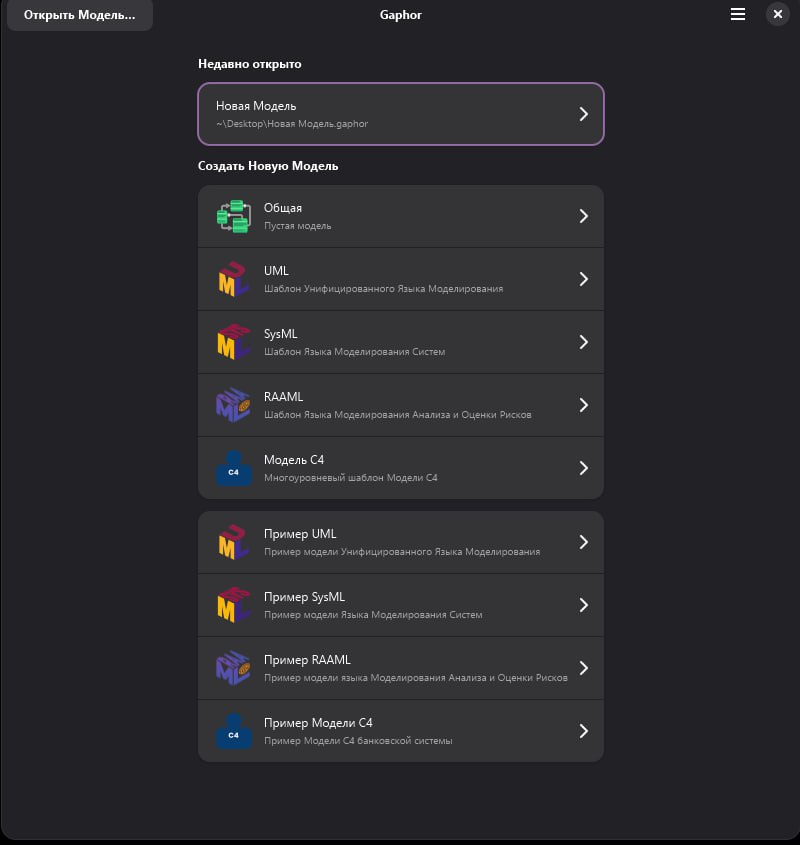
\includegraphics[width=0.78\textwidth]{start.jpg}
    \refstepcounter{figure}
    \caption*{Рисунок \thefigure\ — Стартовый экран шаблонов}
\end{figure}

После того, как шаблон выбран, загружается главное окно Gaphor, и котором можно приступить к моделированию. Мною была выбран шаблон SysML - "Модель навигации". Главное окно Gaphor предсталвено на рисунке 2.
\begin{figure}[H]
    \label{fig:2}
    \centering
    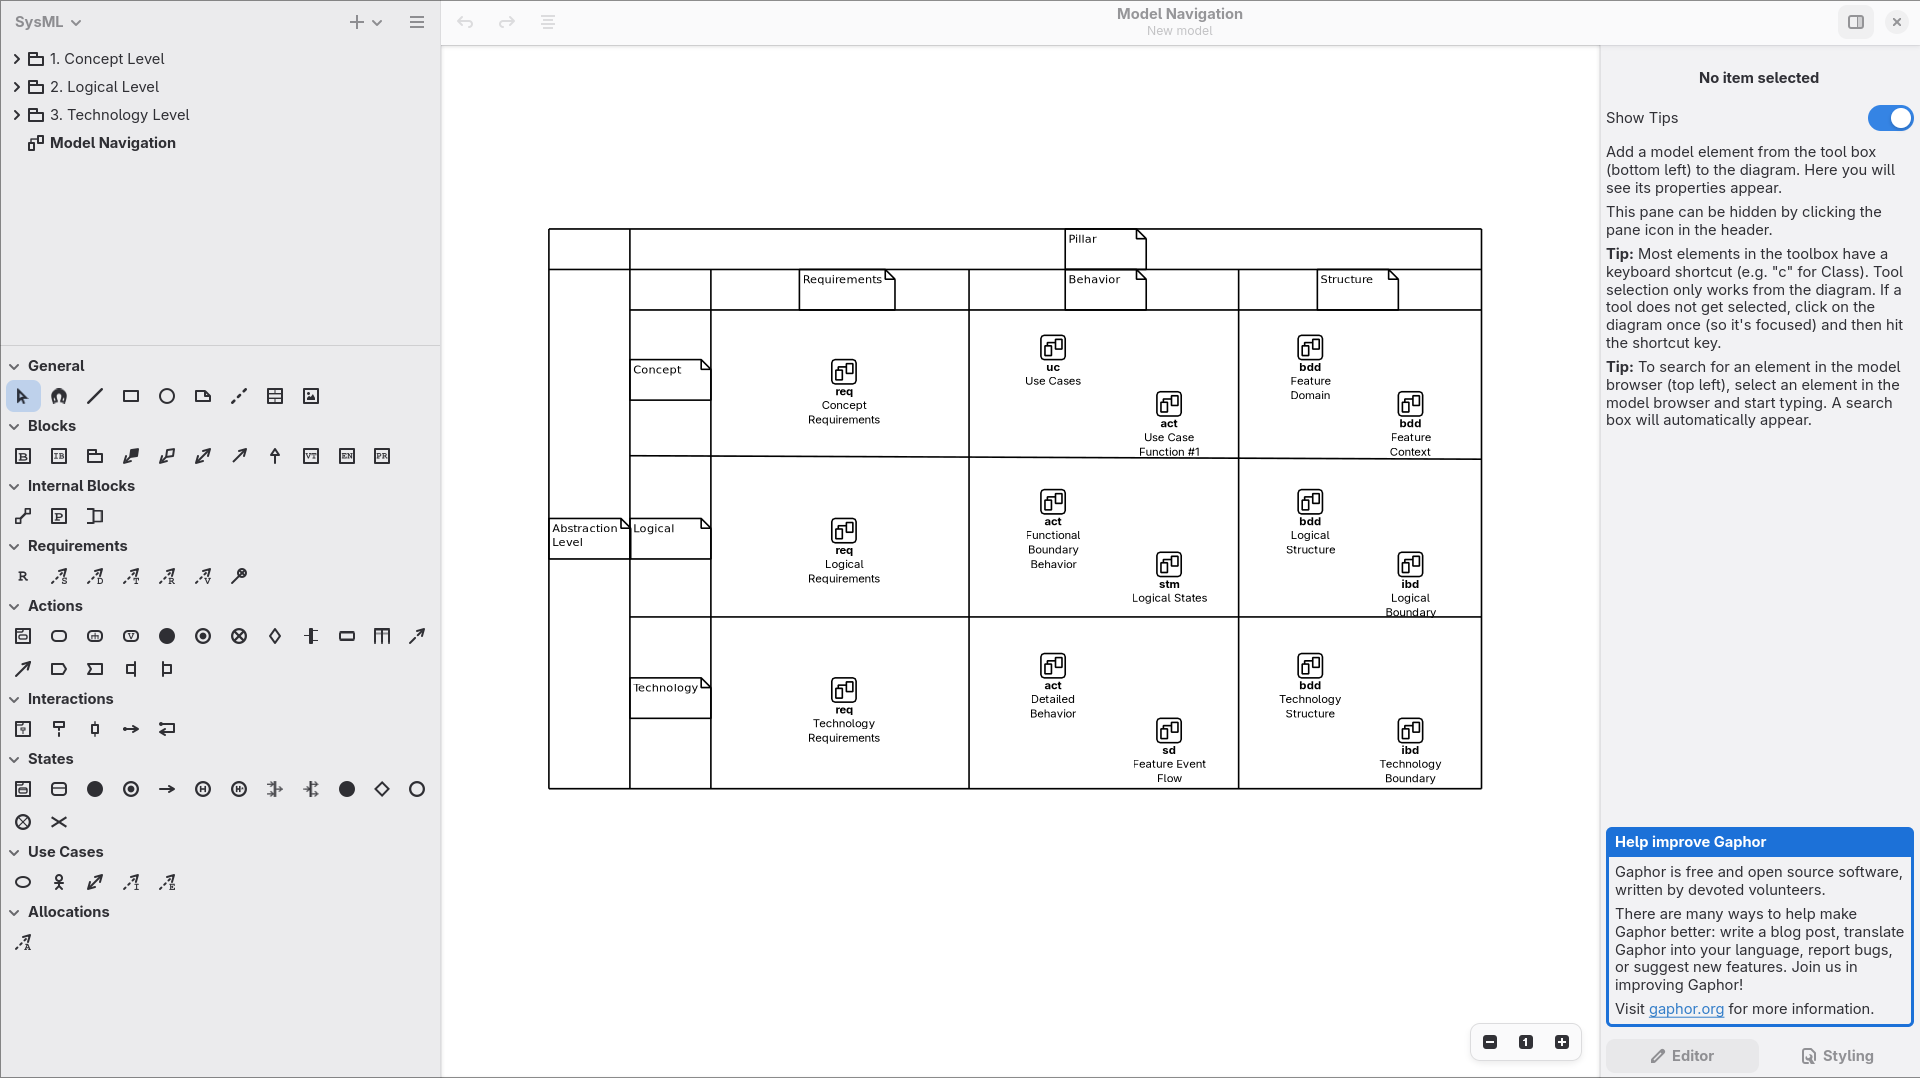
\includegraphics[width=0.78\textwidth]{main.jpg}
    \refstepcounter{figure}
    \caption*{Рисунок \thefigure\ — Главное окно Gaphor}
\end{figure}

    Gaphor автоматически выберет правильный профиль на основе выбранного шаблона, но также можно выбрать другие профили моделирования, если это необходимо, нажав на кнопку рядом с выпадающим меню профиля в верхней части окна.
    Окно Выбора языка моделирования представлено на рисунке 3.
\begin{figure}[H]
    \label{fig:3}
    \centering
    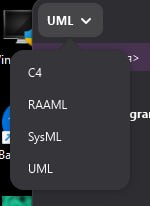
\includegraphics[width=0.78\textwidth]{langs.jpg}
    \refstepcounter{figure}
    \caption*{Рисунок \thefigure\ — Выбор языка моделирования}
\end{figure}

Чтобы выбрать элемент, который хотим разместить, например класс, щелкнем по значку на панели инструментов, а затем снова на диаграмме. Это позволит разместить новый элемент класса на диаграмме и добавить новый класс в модель (он отобразится в браузере моделей).
Части панели инструментов также могут быть свернуты в зависимости от типа моделируемой диаграммы. При необходимости можно развернуть свернутые части панели инструментов.
Область окна с модулями представлена на рисунке 4.
\begin{figure}[H]
    \label{fig:4}
    \centering
    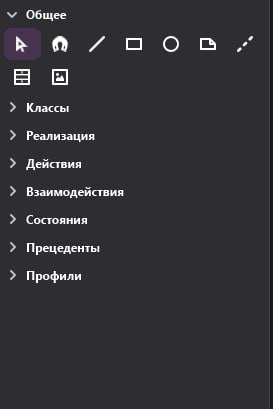
\includegraphics[width=0.78\textwidth]{modul.jpg}
    \refstepcounter{figure}
    \caption*{Рисунок \thefigure\ — Модули}
\end{figure}

Окно свойств выбранного класса представлены на рисунке 5.
\begin{figure}[H]
    \label{fig:5}
    \centering
    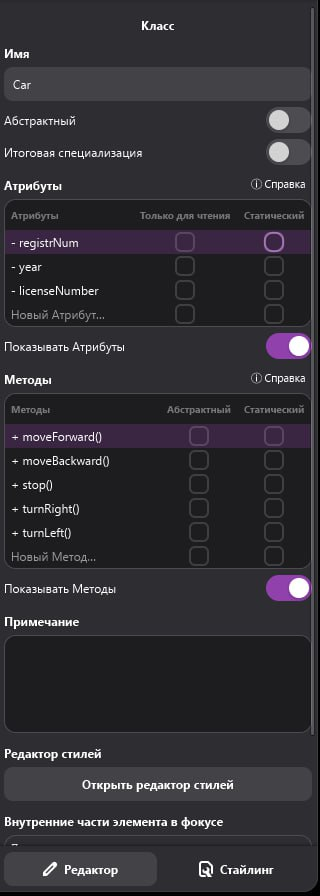
\includegraphics[width=0.78\textwidth]{class.jpg}
    \refstepcounter{figure}
    \caption*{Рисунок \thefigure\ — Свойства класса}
\end{figure}

Стайлинг с помощью CSS представлен на рисунке 6.
\begin{figure}[H]
    \label{fig:6}
    \centering
    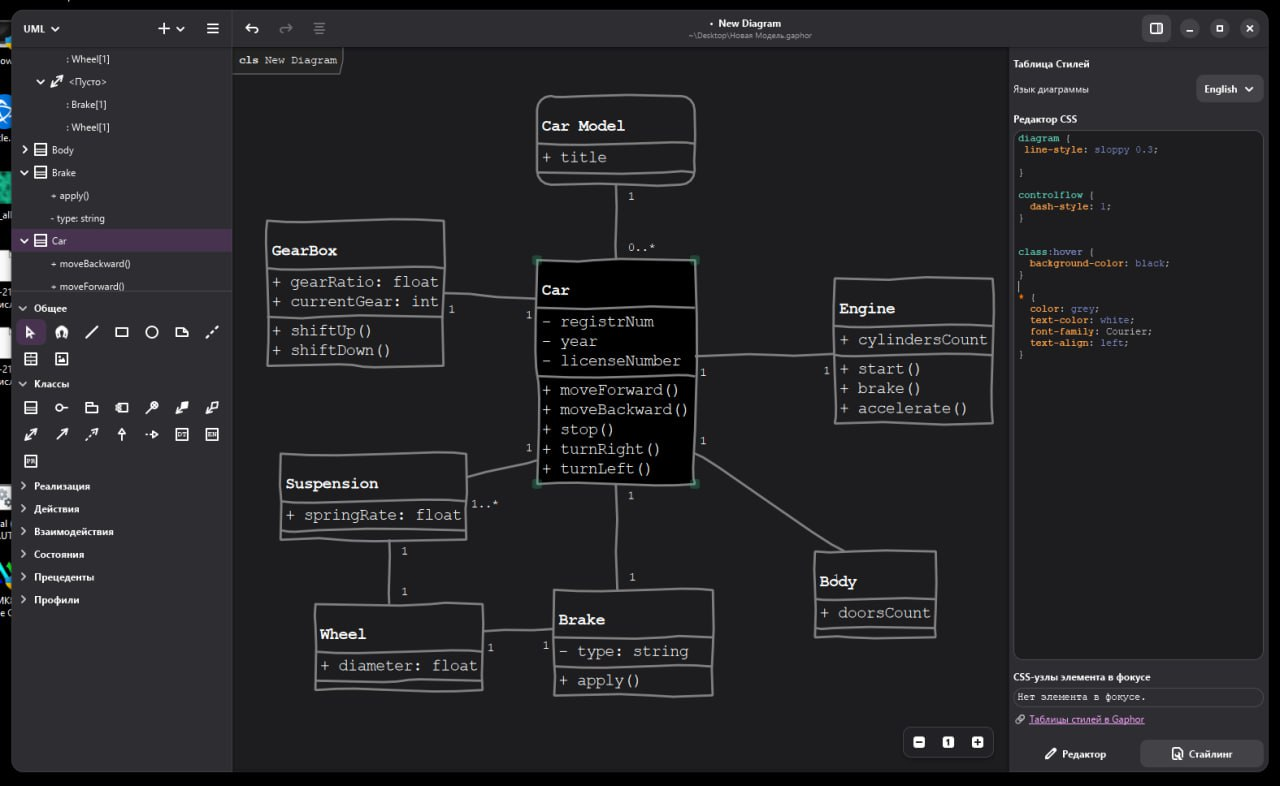
\includegraphics[width=0.78\textwidth]{css.jpg}
    \refstepcounter{figure}
    \caption*{Рисунок \thefigure\ — Стайлинг (CSS)}
\end{figure}


Окно иерархии представлено на рисунке 7.
\begin{figure}[H]
    \label{fig:7}
    \centering
    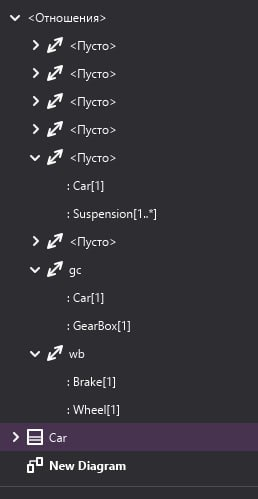
\includegraphics[width=0.78\textwidth]{hierarchy.jpg}
    \refstepcounter{figure}
    \caption*{Рисунок \thefigure\ — Иерархия}
\end{figure}

Окно с подсказкой горячих клавиш представлено на рисунке 8.
\begin{figure}[H]
    \label{fig:8}
    \centering
    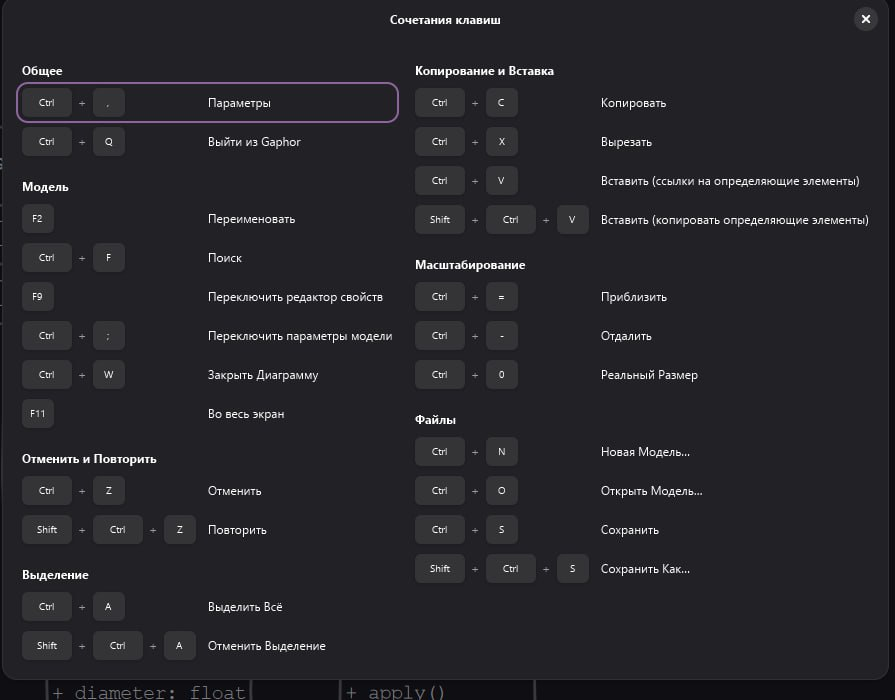
\includegraphics[width=0.78\textwidth]{keys.jpg}
    \refstepcounter{figure}
    \caption*{Рисунок \thefigure\ — Горячие клавиши}
\end{figure}
В программе доступна функция авторасположения элементов на макете.
Результат авторасположения представлен на рисунке 9.
\begin{figure}[H]
    \label{fig:9}
    \centering
    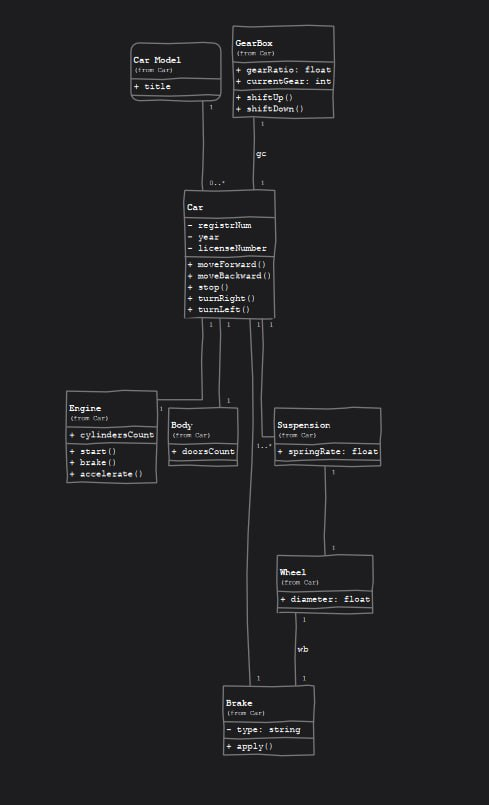
\includegraphics[width=0.78\textwidth]{auto.jpg}
    \refstepcounter{figure}
    \caption*{Рисунок \thefigure\ — Авторасположение}
\end{figure}

Окно с информацией о программе представлено на рисунке 10.
\begin{figure}[H]
    \label{fig:10}
    \centering
    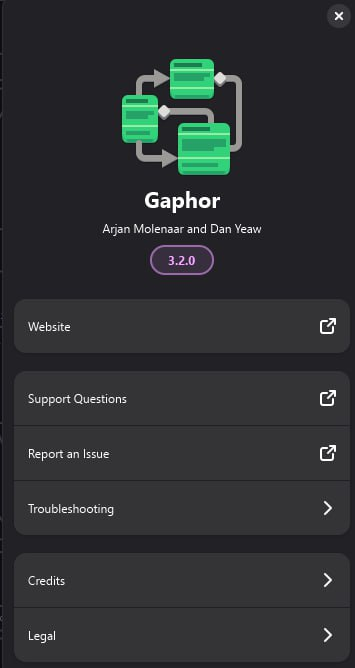
\includegraphics[width=0.78\textwidth]{info.jpg}
    \refstepcounter{figure}
    \caption*{Рисунок \thefigure\ — Информация о программе}
\end{figure}
\newpage

\section{Вывод}
В ходе выполненного индивидуального домашнего задания изучил и поработал с
программой для построения UML/SysML моделей Gaphor.

\end{document}
